\let\negmedspace\undefined
\let\negthickspace\undefined
\documentclass[journal]{IEEEtran}
\usepackage[a5paper, margin=10mm, onecolumn]{geometry}
\usepackage{lmodern} % Ensure lmodern is loaded for pdflatex
\usepackage{tfrupee} % Include tfrupee package
\usepackage[utf8]{inputenc}
\usepackage[T1]{fontenc}

\setlength{\headheight}{1cm} % Set the height of the header box
\setlength{\headsep}{0mm}     % Set the distance between the header box and the top of the text

\usepackage{gvv-book}
\usepackage{gvv}
\usepackage{cite}
\usepackage{amsmath,amssymb,amsfonts,amsthm}
\usepackage{algorithmic}
\usepackage{graphicx}
\usepackage{textcomp}
\usepackage{xcolor}
\usepackage{txfonts}
\usepackage{listings}
\usepackage{enumitem}
\usepackage{mathtools}
\usepackage{gensymb}
\usepackage{comment}
\usepackage[breaklinks=true]{hyperref}
\usepackage{tkz-euclide} 
\usepackage{listings}
\usepackage{gvv}                                        
\def\inputGnumericTable{}                                 
%\usepackage[latin1]{inputenc}
\usepackage{color}                                            
\usepackage{array}                                            
\usepackage{longtable}                                       
\usepackage{calc}                                             
\usepackage{multirow}                                         
\usepackage{hhline}                                           
\usepackage{ifthen}                                           
\usepackage{lscape}
\begin{document}

\bibliographystyle{IEEEtran}
\vspace{3cm}

\title{1.1.5.15}
\author{EE24BTECH11045 - N.Tapasvi}
{\let\newpage\relax\maketitle}
Question:\\
The midpoint of the line segment joining $\vec{A}\myvec{2a\\4}$ and $\vec{B}\myvec{\text{-}2\\3b}$ is $\vec{P}\myvec{1, 2a\\1}$. Find the values of a and b.
\hfill (10,2019)
\\
\solution
\begin{table}[h!]    
  \centering
  \begin{tabular}[12pt]{ |c| c|}
    \hline
    \textbf{Variable} & \textbf{Description}\\ 
    \hline
	$\vec{A}$ & $\myvec{2a\\4}$\\
	\hline
	$\vec{B}$ & $\myvec{-2\\3b}$\\
	\hline
	$\vec{C(Midpoint)}$ & $\myvec{1\\2a+1}$\\
	\hline
	$\vec{a,b}$ & Values to be found\\
\end{tabular}

  \caption{Variables Used}
  \label{tab1-1.9-6}
\end{table}\\
The equations in standard form are:
\[
2a - 0b = 4 \Rightarrow
\begin{bmatrix}
2 & 0 \\
\end{bmatrix}
\begin{bmatrix}
a \\
\end{bmatrix}
=
\begin{bmatrix}
4 \\
\end{bmatrix}
\]

\[
0a + 3b = 6 \Rightarrow
\begin{bmatrix}
0 & 3 \\
\end{bmatrix}
\begin{bmatrix}
b \\
\end{bmatrix}
=
\begin{bmatrix}
6 \\
\end{bmatrix}
\]

We can represent these equations as a matrix:
\[
\begin{bmatrix}
2 & 0 \\
0 & 3 \\
\end{bmatrix}
\begin{bmatrix}
a \\
b \\
\end{bmatrix}
=
\begin{bmatrix}
4 \\
6 \\
\end{bmatrix}
\]

Solving the Matrix Equation.

After soving the equation,the values of a and b are

a=2
b=2
\begin{figure}[h!]
   \centering
   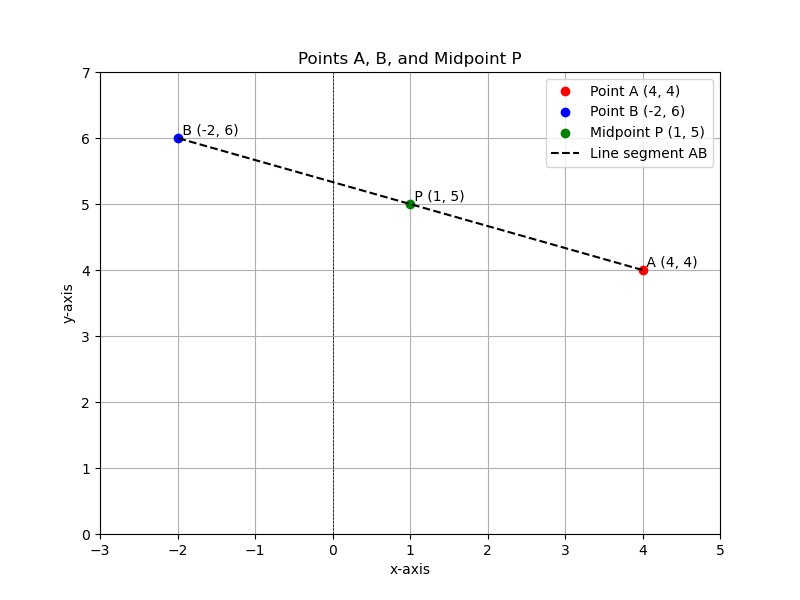
\includegraphics[width=1.15\linewidth]{/home/namala-tapasvi/Figure_1.png}
   \caption{Plot of the points A,B,P}
   \label{stemplot}
\end{figure}
\end{document}

